% !TeX spellcheck = en_GB
\documentclass[main.tex]{subfiles}

\begin{document}
\chapter{Theory and State of the Art}
\lhead{Theory and State of the Art}
\label{chap:theory}
\paragraph{Pretraining and Fine-tuning}
With the advent of deep learning in the field of NLP, models have risen massively in complexity, requiring ever more compute and data.
For instance, LUKE required 30 days of training on 16 NVIDIA V100's \cite{yamada2020luke}, and that model already took advantage of RoBERTa, which was even more demanding to train \cite{liu2019roberta}.
For this reason, the training of a language model is typically divided into two separate tasks:
First, the \emph{pretraining}, in which a model is trained that has little direct practical use but has general language understanding used to produce \emph{contextualized word representations} (CWR's), a construction that will be introduced in section \ref{sec:transformers}
Secondly a \emph{fine-tuning}, or downstream training, in which the pretrained model undergoes further, specialized training for some specific language task, e.g. named entity recognition.

Such pretrained models, producing CWR's, are called \emph{contextualized word representation language models} or \emph{general-purpose language models} \cite[Ch. 2]{birk2020knowledge} and will in this project be referred to simply as \emph{language models}.

\section{Named Entity Recognition}
\begin{enumerate}
    \item Lidt flere eksempler på anvendelser? marrero og særligt danlp har begge en ret udtømmende liste af NER-ting
\end{enumerate}
Natural language processing has the broad goal of algorithmically understanding natural languages such as English and Danish.
To quantify this abstract ideal, understanding is often measured in performance on a set of well-defined language challenges that are expected to require some general understanding.
One such challenge is the task of recognizing \emph{named entities}, rigidly defined real-world objects such as specific persons, locations, organizations, events, products, etc.
The problem of named entity recognition (NER) is to produce an algorithm that can, given a string of characters designating a document of natural language, return an \emph{annotation} which ascribes, to each word in the document, both whether the word is a part of a named entity (NE) and what category of NE the word corresponds to \cite{wiki2021ner}.
For the string
\[
    \text{
        ''Caesar marched on Rome, defying the Senate of the Roman Republic.'',
    }
\]
a correct result could be
\begin{itemize}
    \item \emph{Caesar} is a person,
    \item \emph{Rome} is a location,
    \item \emph{the Senate of the Roman Republic} is an organization,
    \item and all other words are not part of named entities.
\end{itemize}
There are multiple ambiguities in this formulation of the problem but this is a common issue for the problem, as the set of NE types varies between benchmarks and as the definition of a NE is unsettled with possible answers including proper nouns, rigid designators and unique identifiers \cite[Sec. 4]{marrero2013ner}.
For the benchmarks used in this project, the NE categories and annotation formats are introduced in Section~\ref{sec:nerdata} while the evaluation of the performance of NER algorithms is discussed in Section~\ref{subsec:nereval}.

NER is not just used as a benchmark for language understanding:
In the applied field of information retrieval, semantic annotation and question answering systems rely on NER to control the information focus \cite[Sec. 2]{marrero2013ner}.
This task of both research and practical interest was defined in the 90's and has been active and competitive, especially in English where state of the art (SOTA) methods achieve close to human performance on some classic benchmarks \cite{wiki2021ner, marrero2013ner}.
Researchers argue, however, that the task is not yet solved as the generalization of the statistical algorithms fitted to one NER dataset to new examples is poor \cite[Sec. 7.2]{marrero2013ner}.

The SOTA on English NER benchmarks moves quickly, but almost all algorithms currently (June 2021) achieving high scores in common benchmarks are deep neural networks and of the transformer architecture in particular \cite{ruder21ner, pwc21ner}.

\section{Embeddings, Tokenization and The Transformer}
\label{sec:transformers}
\begin{enumerate}
    \item Mere plads til BERT?
\end{enumerate}
Danish is, compared to English, a low resource language:
The world's Danish speaking population is smaller than the English speaking population of large cities, naturally resulting in significantly fewer and smaller available text datasets, and in less attention from both researchers and practitioners.
While pushing the performance of current natural language processing (NLP) algorithms to their limits is much more difficult in low resource languages, the field of applied NLP in Danish has adopted many of the deep learning developments of recent years.

Especially models based on the transformer neural network architecture \cite{vaswani2017att} currently dominate the Danish NER scene \cite{danlp2021}.
To understand the transformer, a closer look is first taken at traditional word embeddings and their shortcomings.

\paragraph{Word embeddings}
Word embeddings are one of the most ubiqitous tools in the NLP toolbox and come in many variants, all sharing the general idea of mapping a word token to a real-valued vector representation corresponding to a semantic condensation of the word.
When using the term \emph{embeddings}, we refer to the static, uncontextualized representations such as the \emph{fasttext}-based, 300-dimensional, Danish embeddings released by Edouard Grave et al. \cite{grave2018learning}.

One of the challenges in language modelling is that many words change their meaning completely depending on the context in which they appear.
Consider for instance, the sentences ''The mouse and the elephant'' and ''Please left-click using the mouse''.
''mouse'' appears identically in both sentences, but with widely different meanings, which static embeddings have a hard time modelling.
In the latent space of the embeddings, one would expect ''mouse'' to be close to other species from the animal kingdom, but also close to computer parts.
This would in turn cause computer parts to be placed close to animals, which is not ideal.
This issue with embeddings is where the transformer comes in.

\paragraph{The Transformer}
Introduced by Ashish Vaswani et al. in 2017 \cite{vaswani2017att}, the goal of the transformer is to produce \emph{contextualized word representations} (CWR) given static, but learned embeddings.
CWR's are similar to embeddings in that they are real-valued vector representations of words but they also take the document context into account

Transformers are not the first attempt to solve this problem of producing effective CWR's.
Older architectures such as recurrent neural networks \cite[Ch. 10]{Goodfellow-et-al-2016} and in particular long short-term memory networks \cite{hochreiter1997lstm} have yielded strong results, but we argue that they have three key weaknesses:
First of, they only include context up to the given word, and secondly, they struggle with long-term dependencies due to their sequential nature resulting in poor information preservation \cite{Goodfellow-et-al-2016}.
Finally, the sequentiality of their calculations also limits how parallelized training and inference can be.
The first issue has been solved by the introduction of bi-directional versions of these network types \cite{schuster1997birnn}.
The second issue of long-term dependencies and the third of parallelizability is what the transformer seeks to tackle.

Both of these issues are solved by the attention mechanism.
Instead of sequentially letting each token update the state as in traditional language models, the relevance of all tokens to all other tokens are calculated simultaneously, which can be done in parallel while not loosing any information to an iterative state update.

The transformer uses an encoder-decoder structure with the encoder producing the CWR's.
The encoder is made of several attention blocks feeding into each other with feed forward networks and layer normalizations in between.
The attention blocks are each made up of three learnable matrices: the query, key, and value matrices.
The word embeddings are structured in a single matrix with token embeddings in the rows and multiplied upon the three matrices before the attention scores calculated.
This allows every token to be considered simultaneously, independently, and equally, solving both the described issues.
\cite{vaswani2017att}

Models based directly on the transformer have been trained on very large corpora to produce English language models such as BERT \cite{devlin2019bert}, RoBERTa \cite{liu2019roberta} and GPT-3 \cite{brown2020language} that have achieved SOTA in several downstream language tasks.
BERT is the first model to use the masked language model pretraining objective as it is employed by e.g. RoBERTa and LUKE.
Early transformer based models such as OpenAI's GPT \cite{rashford2018gpt} use a unidirectional pretraining task, letting only tokens appearing to the left of the token to predict have any impact.
BERT instead masks some tokens in the given sequence and allows all tokens to attend to all other tokens when predicting the masked ones -- this is what is known as a masked language model.
BERT achieved SOTA on a large amount of downstream tasks such as the important question answering task and has been described as revolutionary for its impact on NLP \cite{raj2019bert}.
Figure \ref{fig:transformer-bert} shows both the transformer architecture and the BERT pretraining and fine-tuning.
\begin{figure}[H]
    \centering
    \begin{minipage}{0.35\linewidth}
        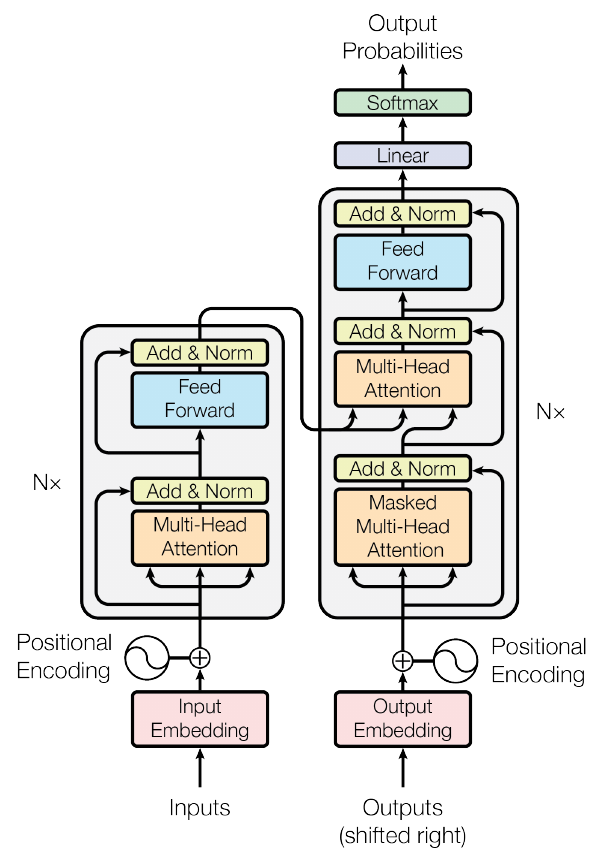
\includegraphics[width=\linewidth]{imgs/transformer}
    \end{minipage}\hfill
    \begin{minipage}{0.64\linewidth}
        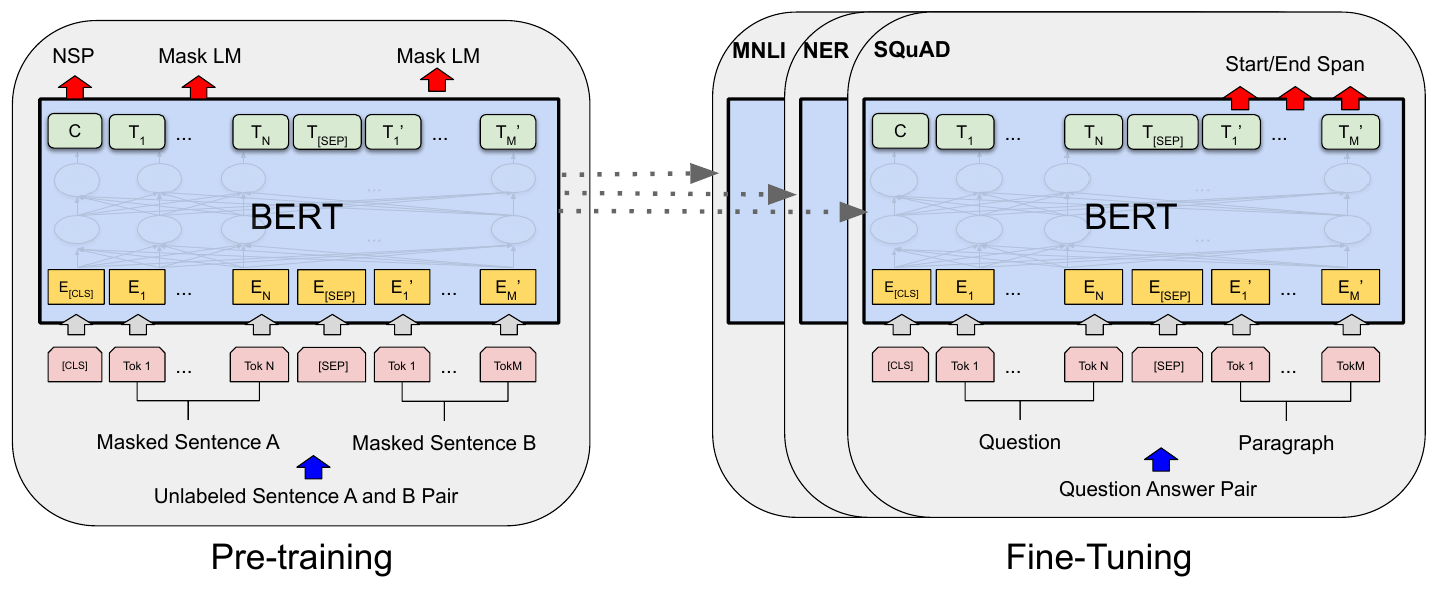
\includegraphics[width=\linewidth]{imgs/bert}
    \end{minipage}
    \caption{
        To the left, the transformer architecture is shown as proposed by Vaswani et al. \cite{vaswani2017att}
        The right-hand side shows the BERT pipeline as introduced by Devlin et al. \cite{devlin2019bert}
        Both Figures are taken from their respective papers.
    }
    \label{fig:transformer-bert}
\end{figure}\noindent

\paragraph{Tokenization}
The input to these language models must naturally be sequences of words.
A naïve approach is to regard all unique words seen in corpus as tokens.
However, the fact that multiple possible augmentations of same word can be met makes this a suboptimal method.
A verb, for example, still carries much of the same meaning between conjugations, but the naïve solution would require learning a new embedding for each form.
While this might be solved by lemmatizing words to their stems, this introduces a problem of information loss.

A more effective way of tokenizing has been presented by Sennrich et al. \cite{sennrich-etal-2016-neural} that uses the byte-pair encoding (BPE) compression algorithm.
This method produces a token vocabulary of a given size from the corpus where each token is either a full word or a subword.
BERT uses the WordPiece BPE token vocabulary which contains 30,000 tokens that have been learned with heuristic tokenization rules \cite{wu2016tokenize} \cite{devlin2019bert}.
Radford et al. \cite{Radford2019gpt2} modify BPE tokenization for the GPT-2 transformer such that splits are made on the byte level rather than on the character level, which works better on corpora containing many non-ASCII characters.
This method is used by RoBERTa to produce a token vocabulary of size 50,000 \cite{liu2019roberta}.
LUKE directly uses RoBERTa's tokenizer when dealing with words \cite{yamada2020luke}.

\section{Deep Natural Language Processing in Danish}
\label{sec:nlpda}
As mentioned earlier, static embeddings are a core part of many NLP pipelines and have been for a long time.
In the large, open source NLP frameworks \emph{SpaCy} \cite{honnibal2020spacy} and \emph{Flair} \cite{akbik2019flair}, which also release pretrained Danish models, the embeddings interact with different, ever-improving language models.
This has successfully resulted in SOTA on multiple Danish NLP tasks.
The Alexandra Institute, a Denmark based AI research and development organization, release versions of both Flair and SpaCy fine-tuned on a number of benchmarks, including NER, and acquire close to SOTA performance using these.
The benchmarks, results and fine-tuned Danish models are released as a part of their open source DaNLP project gathering resources for Danish NER \cite{danlp2021}.
Another application of exsting NLP frameworks was performed by Kenneth Enevoldsen, Center of Humanities Computing, Aarhus University in releasing the model \emph{DaCy}, based on version 3 of SpaCy \cite{enevoldsen2020dacy}.

In Danish, the most significant, pretrained language model is in our estimation a Danish version of BERT, released by the company BotXO in 2019 \cite{botxo2019dabert} .
This model, in the following called \emph{da-BERT}, is produced by pretraining the base version of BERT \cite{devlin2019bert} on 10 GB of Danish text predominantly acquired from web scrapes.
The da-BERT model has been fine-tuned on most Danish benchmarks in the DaNLP project and consistently yield top results \cite{danlp2021, hvingelby2020dane}.
The model and its tokenizer are trained on lowercased text.

Another, more recent, Danish transformer is the adaption of the more resource efficient language model Electra to Danish under the name Ælæctra by Malte Hømark-Bertelsen, KMD and Aarhus University \cite{bertelsen2020lctra}.
NER fine-tuned versions of Ælæctra and some multilingual transformers have been released by Ekstra Bladet Analyse under the project \emph{NER for Danish} (NERDA) \cite{kjeldgaard2020nerda}.

Of this plethora of Danish language models and NLP frameworks, the current (June 2021) state of the art on central NER benchmarks is, according to DaNLP, the 2021 newcomer DaCy which surpassed DaNLP's fine-tuned da-BERT model which was SOTA at the beginning of this project \footnotemark.
\footnotetext{
    A Table of the results can be seen at the DaNLP repository at \url{https://github.com/alexandrainst/danlp} under \code{docs/docs/tasks/ner.md}.
}
These results are reproduced and compared with DaLUKE in the project.
The NER benchmark will be presented in Section \ref{subsec:daNERdata}, the reproduction method in Section \ref{sec:exidan}, and the results in Section \ref{sec:nerres}.

Finally, the NLP scene of a language is much more than the public, pretrained models:
The available rule-based tools, corpora and other language resources are instrumental in developing practical NLP pipelines.
One pipeline supplying multiple of these resources is the IT University of Copenhagen project DKIE, also including a NER model \cite{derc2014dkie}.
A 2019 paper by NLP researchers at the same university surveyed the availability of such tools and highlight a lack of practical resources and datasets \cite{kirkedal2019lacunae}.
Other overviews of Danish NLP resources include those published by the Alexandra Institute at DaNLP \cite{danlp2021} and the comprehensive list maintained by Finn Årup Nielsen, DTU Compute \cite{arup21awesome}.

\section{Deep, Knowledge-enhanced NLP}
The combination of statistical methods and explicit human crafted domain knowledge was the SOTA in many natural language processing (NLP) tasks in the 1990's and up into the 2000's \cite[Sec. 22.5]{russell2016ai}.
As with most other fields of AI, the emergence of performant deep learning methods disrupted NLP in the 2010's, popularizing the methodology of using deep architectures such as recurrent neural networks or transformers as general purpose language models that can be fine-tuned to a number of different tasks \cite{otter18dlnlp}.
This approach rarely includes any modelling of knowledge that is not induced implicitly by the contextual representations generated during pretraining on an unannotated text corpus.

The Defense Advanced Research Projects Agency (DARPA) identify the future wave of AI as one of \emph{contextual adaption}; a combination of deep learning for perception and latent representations and symbolic modelling methods \cite{darpa17ai}.
In NLP, knowledge-enhancing deep neural networks is not just an idea for the future:
Several approaches using explicit knowledge to improve pretrained contextual word representations (CRW's) have been presented in recent years, a subset of which will be summarized here.

\subsection{Static, Separate Knowledge Graphs}
A direct way to use explicit knowledge is to maintain a separate representation of facts which can be incorporated into both pretraining and inference of deep language models.
This representation is often called a knowledge base (KB)  -- or knowledge graph (KG) if the relational facts or entities are modelled.

In 2019, \emph{Enhanced Language Representation with Informative Entities}, ERNIE, was introduced by a Beijing team \cite{zhang2019ernie} looking to ''enhance language representation  with  external  knowledge'' \cite[1]{zhang2019ernie} by recognizing mentions of named entities in given text and retrieving their positions in a separate knowledge graph.
The query from the knowledge graph is encoded into knowledge embeddings which are taken as input for a BERT-based dual transformer architecture.
The model was during training required to fill in randmoly masked named entities in given sequences using the KG.
ERNIE was not evaluated on named entity recognition in the original paper, but was evaluated on the \emph{General Language Understanding Evaluation} benchmark \cite{wang2018glue} where it did not outperform BERT.

Later in 2019, a similar idea was proposed in \emph{Knowledge Enhanced Contextual Word Representations} where the model \emph{KnowBert} \cite{peters2019knowbert} was shown to outperform ERNIE and BERT in knowledge related tasks, though GLUE or NER was not tested.
Here, the key addition was the Knowledge Attention and Recontextualization (KAR) component which allows information to retrieved from multiple KG's of different forms such as WordNET and Wikipedia and represented within the BERT encoder.

In KnowBert, though the KAR weights were trained, the KG was only used for encoding fixed facts for the model.
The \emph{Knowledge Graph Language Model} (KGLM) presented in \emph{Barack’s Wife Hillary: Using Knowledge Graphs for Fact-Aware Language Modeling} \cite{logan2019barack} employs a more dynamic use of the knowledge graph.
The model uses the same approach to representing knowledge graph facts as ERNIE, but also builds a local graph on the sequence level which is grown by a generative model with each new token.
The paper presents improved fact completion compared to GPT-2 and further analysis has shown that the overall fact completion of KGLM is comparative to KnowBert, though they perform very differently from domain to domain, with KGLM being most dependent on the used knowledge graph \cite{birk2020knowledge}.

\subsection{Pretraining Augmentations}
A strength of the statistical, deep approach that implicitly models knowledge is the potential for generalizable results:
You do not need a new domain specific KG for every application if enough general knowledge has been caught in your weights.
Motivated by the hope of this elusive generalizability, a number of methods have been proposed to enhance specifically the pretraining of language models to better have handle factual knowledge.
LUKE, the subject of this project, is one of these attempts.

An example of this weaker knowledge modelling is found in the 2019 model \emph{KEPLER: A Unified Model for Knowledge Embedding and Pre-trained Language Representation} \cite{wang2021kepler} where downstream inference can be performed without any additional resources other than the transformer structure itself.
The knowledge enhancement of this BERT-based language model is, however, in the pretraining where the model optimizes over a joint task of both performing masked language modelling (MLM) and a novel knowledge graph objective requiring the model to learn knowledge embeddings.
KEPLER does not improve GLUE performance from RoBERTa \cite{liu2019roberta} from which it was initialized, but beats both classical language models and knowledge enhanced ones such as ERNIE and KnowBERT on a number of knowledge related tasks.

This idea of pretraining a transformer both for MLM and for a new knowledge-guided task has been taken up multiple times, including in LUKE.
\emph{WKLM}, presented in 2019 in \emph{Pretrained Encyclopedia: Weakly Supervised Knowledge-Pretrained Language Model} \cite{xiong2019wklm}, uses the English Wikipedia, taking hyperlinks to be entities, and trains an unaltered BERT architecture jointly on MLM and on a task involving identifying the randomly replaced entity in a sequence.
\emph{KALM}, published after LUKE in \emph{Knowledge-Aware Language Model Pretraining} \cite{corby2020kalm}, also keeps the core language model architecture, in this case GPT-2, unchanged, adding a separate entity tokenizer and entity embedding layer for an entity prediction pretraining task.

Though these models achieve good performance, with WKLM surpassing BERT and ERNIE on some question answering and entity related benchmarks, and KALM outperforming GPT-2 on some knowledge related zero-shot tasks, the 2020 article \emph{K-Adapter: Infusing Knowledge into Pre-Trained Models with Adapters} \cite{wang2020kadapter} raises a concern with the approach.
According to the authors, the idea of knowledge-augmenting the pretraining task and then updating the entire model limits the ability to inject versatile knowledge and sets up a heterogeneous learning problem resulting in entangled parameters that are hard to investigate.
The model \emph{K-Adapter} instead uses ''adapters'', add-ons for the transformer structure, which are pretrained for different knowledge tasks while the base RoBERTa parameters are not updated.
The resulting model outperforms BERT, WKLM, ERNIE, KEPLER and KnowBERT on central knowledge related tasks.

Another issue, raised more recently, with this jungle of knowledge enhanced models is that they do not unify generative and discriminative tasks, limiting their generalizability to fewer downstream tasks.
This is voiced in \emph{KgPLM: Knowledge-guided Language Model Pretraining via Generative and Discriminative Learning} \cite{he2020kgplm} where the model KgPLM, pretrained by both generating masked entities and discriminating replaced ones, is proposed as a solution.

Which of the knowledge-enhanced models result in the best general performance for practitioners is beyond the scope of this project, as the continuous improvement of many of the models and large amount of different benchmarks used in the articles makes direct comparisons of general language understanding ability challenging.
On all benchmarks tested by the LUKE team \cite{yamada2020luke}, none of the above models have presented higher scores than LUKE \cite[Sec. 4]{yamada2020luke}.


\section{LUKE}
\label{sec:LUKE}
LUKE (Language Understanding with Knowledge-based Embeddings) is a language model introduced by Yamada et al. in November of 2020 \cite{yamada2020luke}.
As the model is applied in this project, key properties of the architecture and pretraining methodology are presented in this section.

As other new models discussed previously, LUKE builds on the BERT transformer architecture \cite{devlin2019bert}, adding a knowledge-enhancing pretraining task.
But the LUKE encoder does not only produces contextualized word representations (CWR); 
\emph{entities} are also represented by the encoder by mapping each entity to the same latent space as the words.
In the pretraining of LUKE, entities correspond to Wikipedia articles.

Yamada et al. show that this approach leads to SOTA results on a number of entity-related tasks, such as NER, and argue that the LUKE approach mitigates the following issues with existing methods:
\begin{itemize}
    \item Existing CWR's cannot represent spans of multiple words which requires more downstream learning for language tasks in which word spans are important.
    \item While transformers are good at capturing relationships between single words, they have difficulty modelling such relationships between sequences of words, of which entities often consist.
    \item Finally, the word-based pretraining task is not suited for producing entity-level representations, as the masked language model (MLM) mostly learns to predict single words rather than entire entity spans.
        An example is predicting ''Rings'' in ''We watched Peter Jackson's The Lord of the [MASK]'', where predicting the single word is clearly easier than predicting the entire entity.
\end{itemize}
The LUKE idea is to consider entities as first-class citizens of text documents along with words, maintaining vocabularies of both entity and word tokens.
\subsection{Architecture}

\paragraph{Input Tokenization}
An input example for LUKE consists both of a sequence of words and a set of entities mentioned in the document, such as:
\begin{itemize}
    \item ''Biden is oldest president of the United States to date.''
    \item $\{\text{\emph{Joe Biden} at word \#1}, \text{\emph{The United States of America} at words \#7-8}\}$.
\end{itemize}
For use of LUKE, the text sequence is tokenized into $m$ subword tokens using the normal tokenizer of RoBERTa, the transformer on which LUKE is based.
The entities are converted to $n$ entity tokens; integer values corresponding to indeces in a vocabulary of known, named entities.
The positions of the entities are included in the further inference as \emph{position ids}.

\paragraph{Entity Embeddings}
The subword tokens are forward passed through the same, static word embedding architecture as that of BERT which outputs $m$ vectors of dimension $H$ for each subword.
For the entity and entity position tokens, the new additions to the inference, a similar component which maps id's to $n$ vectors, also $\in \RR^H$.
These are called entity embeddings and are computed using trainable lookup Tables, which, for the entity id case, corresponds to the entity vocabulary.

The produced word and entity embeddings are concatenated to a matrix $\in \RR^{(n+m)\times H}$.

\paragraph{Transformer}
The representations of words and entities are forward passed through a transformer operating on the entire sequences of embeddings without distinction between words and entities.
This component is dubbed the encoder and, after $N$ attention blocks with same input and output dimensionality, outputs the final contextualized $H$-dimensional representations:
The first $m$ correspond to words and the last $n$ to entities.
The main LUKE model, LUKE large, has, following BERT, $N=24$, $H=1024$

After the computation of the representations, the model can be extended with a decoder consisting of bi-directional classifications heads for pretraining, or it can be extended with linear layers for downstream tasks.
\begin{figure}[H]
    \centering
        \begin{tikzpicture}[shorten >=1pt,->,draw=black!90]
\tikzstyle{every pin edge}=[<-,shorten <=1pt]
\tikzstyle{path} = [ultra thick]
\tikzstyle{neuron}=[circle,fill=black!25,minimum size=17pt,inner sep=0pt]

\tikzstyle{shared neuron}=[neuron, fill=purple!90];
\tikzstyle{word neuron}=[neuron, fill=blue!90];
\tikzstyle{entity neuron}=[neuron, fill=red!90];

\tikzstyle{annot} = [text width=10em, text centered]

\node[annot] (I) at (-2, 0) {\footnotesize Text sequence with annotated entities};

\node[word neuron] (T-W) at (0, 2) {};
\node[entity neuron] (T-E) at (0, -2) {};
\node[annot, above of=T-W, node distance=1 cm] {Word tokenizer};
\node[annot, below of=T-E, node distance=1 cm] {Entity tokenizer};

\path (I) edge (T-W);
\path (I) edge (T-E);

\node[word neuron] (E-W) at (4, 2) {};
\node[entity neuron] (E-E) at (4, -2) {};
\node[annot, above of=E-W, node distance=1 cm] {Word embeddings};
\node[annot, below of=E-E, node distance=1 cm] {Entity embeddings};

\path (T-W) edge (E-W);
\path (T-E) edge (E-E);

\node[annot] at (2, 2.25) {\footnotesize $m$ subword ids};
\node[annot, text width=5em] at (2, -2) {\footnotesize $n$ entity and position ids};

\node[rectangle, draw = black,
    text = white,
    align=center,
    fill = Plum,
    minimum width = 4cm,
    minimum height = 2cm
    ] (T) at (6,0) {Transformer:\\\(24\times\text{attention}\)};

\path (E-W) edge (T);
\path (E-E) edge (T);

\node[annot, text width=4em] at (5.25, 1.5) {\footnotesize $\mathbf w_{1, \ldots, m}$};
\node[annot, text width=4em] at (5.25, -1.5) {\footnotesize $\mathbf e_{1, \ldots, n}$};

\node[annot, text width=1em] at (9,0) {\footnotesize
    $\begin{bmatrix}
    \textcolor{blue!90}{\mathbf x_1}     \\
    \textcolor{blue!90}{\vdots}  \\
    \textcolor{blue!90}{\mathbf x_{m}}   \\
    \textcolor{red!90}{\mathbf x_{m+1}} \\
    \textcolor{red!90}{\vdots}  \\
    \textcolor{red!90}{\mathbf x_{m + n}}
    \end{bmatrix}
    $
};
\path (T) edge (8.75, 0);

\end{tikzpicture}

    \caption{
        Overview of the LUKE pipeline from annotated text to contextualized representations of both words and entities.
        $w_i, e_i, x_i$ all reside $\in \RR^H$ with $H=768$ in the LUKE implementation.
    }
    \label{fig:luke}
\end{figure}\noindent

\paragraph{Transfer Learning}
The word/entity duality of LUKE means that a large part of the model performs the same task as the conventional word-based language models.
For this reason, the word embeddings in LUKE follow the BERT architecture and Yamada et al. initialize these embeddings to those found in RoBERTa.
In the pretraining of Yamada et al., the encoder of LUKE is also equivalent with that of BERT and is initialized using the weights of RoBERTa.


\paragraph{Entity-aware Self-attention}
\label{subsubsec:entityaware}
Yamada et al. present a entity-related change to the BERT encoder architecture in the query metchanism of the attention scorer \cite[Sec. 3.2]{yamada2020luke}.

For the attention between token $i$ and token $j$ with the representations $\mathbf x_i, \mathbf x_j$, a core part of the normal transformer attention mechanism is to compute the following scalar:
\begin{equation}
    q_{ij} = \mathbf x_j^\top \mathbf Q \mathbf x_i,
\end{equation}
where $\mathbf Q\in \RR^{H\times H}$ is a learnable weight called the query matrix \cite[Sec. 3.2.1]{vaswani2017att}.

In LUKE, the tokens $\mathbf x_i$ might either be words or entities.
To handle this explicitly, the idea of \emph{entity-aware self-attention} changes the computation of the query attention scalar $q_{ij}$ to
\begin{equation}
    q_{ij} = 
    \begin{cases}
    \mathbf x_j^\top \mathbf Q_{w2w} \mathbf x_i  & \text{if both $\mathbf x_i$ and $\mathbf x_j$ are word tokens}\\
    \mathbf x_j^\top \mathbf Q_{w2e} \mathbf x_i & \text{if $\mathbf x_i$ is word and $\mathbf x_j$ is entity}\\
    \mathbf x_j^\top \mathbf Q_{e2w} \mathbf x_i & \text{if $\mathbf x_i$ is entity and $\mathbf x_j$ is word}\\
    \mathbf x_j^\top \mathbf Q_{e2e} \mathbf x_i & \text{if both $\mathbf x_i$ and $\mathbf x_j$ are entity tokens}
    \end{cases}.
\end{equation}
LUKE, however, is not pretrained using this mechanism, but for the fine-tuning tasks, Yamada et al. show in ablation experiments that using this addition consistently yields better performance \cite[Sec. 5.2]{yamada2020luke}.
This new mechanism, theorized to improve entity knowledge by Yamada et al., was  not used in preatraining with the following explanation:
''We perform pretraining using the original self-attention mechanism rather than our entity-aware self-attention mechanism because we want an ablation study of our mechanism but can not afford to run pretraining twice'' \cite[Sec. 3.4]{yamada2020luke}.

\subsection{Pretraining}
\label{subsec:lukepre}
Yamada et. al perform the pretraining of LUKE by extending the MLM task of BERT \cite{devlin2019bert}.
Where BERT is trained to predict randomly masked words, LUKE is trained to predict both randomly masked words and entities, such as
\begin{itemize}
    \item ''Franklin Roosevelt did not [MASK] to see the [MASK] of WWII.''
        \subitem Truth: ''live'', ''end''.
    \item $\{\text{\emph{[MASK]} at words \#1-2}, \text{\emph{World War II} at word \#11}\}$
        \subitem Truth: ''Franklin D. Roosevelt''.
\end{itemize}
Following RoBERTa \cite{liu2019roberta}, subword tokens making up 15\pro\ of full words in each sequence are randomly replaced with the [MASK] token.
Of these, 10\pro\ are unmasked again, and another 10\pro\ are replaced by a random token from the vocabulary instead of [MASK].
Similarly, 15\pro\ of entity tokens are replaced with [MASK], but none of these are unmasked or replaced with random entities.
The model is then trained to predict all subword tokens.
From these, the model is to classify the tokens at the mask positions in both sequences.
The model parameters are then updated by the stochastic gradient optimization algorithm known as \emph{Adam with weight decay fix} (AdamW) \cite{hutter2019adamw}.

For a batch of size $ N $ and $ C $ classes, the model produces a matrix of size $ N\times C $ where $ X_{i, j} $ is the class score for class $ j $ for the $ i $'th example in the batch.
For each of the two classification tasks, the cross entropy loss $ l $ is then calculated as
\begin{equation}\label{eq:crossentropyloss}
    l = \frac{1}{N} \sum_{i=1}^N \left(
        -X_{i, c_i} + \log \sum_{j=1}^C \exp X_{i, j}
    \right),
\end{equation}
where $ c_i $ is the true class of the $ i $'th example \cite{pytorchcel}.
The total loss is then calculated as the sum of individual losses for both tasks.

Yamada et al. \cite{yamada2020luke} use weight decay for the entire model barring bias and layer normalizations.
According to Krogh and Hertz \cite{krogh1991weight}, weight decay improves generalizability in feed-forward networks.
This is due to the suppression of irrelevant parameters, letting the smallest possible parameters solve the problems.
Larger parameters naturally lead to larger sensitivity to noise and thus poorer generalization.

\paragraph{Entity Mask Prediction Head}
For the entity pretraining task, LUKE is equipped with another classifier structure in addition to the masked language model prediction head inherited from BERT.
This new prediction head follows the architecture of the masked word scorer just operating on the entity representations.
The masked entity tokens are thus scored as corresponding to one of the entities in the entity vocabulary by two linear layers between which an activation function and layer normalization are placed.

\subsection{Fine-tuning for Named Entity Recognition}
\label{subsec:fine-tuning-theory}
Yamada et al. base their NER fine-tuning on the method from Sohrab and Miwa \cite{sohrab2018nestedner}.
All possible spans over the entire sequence (or $n$-grams) are calculated and saved as entity candidates.
Spans longer than 16 words and spans that cross sentence boundaries are discarded.
Each span along with the text in which it appears is saved as a NER example.

An example is forward passed through LUKE by marking the candidate entity with the [MASK] entity id.
For each named entity candidate, the computed representation of this [MASK] entity and the CWR's of the first and last word tokens in the span are concatenated.
[MASK] is used as NE candidate as this it was used for a similar prediction task in the pretraining.
Only [MASK], and [PAD], are used out of all the entity embeddings that LUKE contains.

The combined representation from the pretrained model is then given to a single linear layer that learns to classify the entity as either a non-entity or one of the classes in the dataset.
For a dataset with $ n $ classes, the learning problem is then an $ n+1 $ class classification task.
The loss is calculated as the cross entropy loss between the predicted class scores and the true class scores using equation \eqref{eq:crossentropyloss}.
Both the full pretrained model and the linear classifier are fitted.
An issue with the $ n $-grams is the large amount of overlaps between spans.
This is solved by greedily selecting spans based on the class scores from the classifier.
Thus, if two (partially) overlapping spans both are predicted to cover an entity, only the one with the highest score is kept, while the other is predicted to be a non-entity.

Following BERT \cite{devlin2019bert}, the maximal document context is included in the target document, allowing each entity prediction to use as much context as the dataset provides, limited only by the maximum of 512 subword tokens given to LUKE.
This plays to the strengths of the transformer, which is good at retaining attention over long sequences of text \cite{vaswani2017att}.
\cite{yamada2020luke}

\end{document}
